\documentclass{beamer}
\usepackage{enumerate}
\usepackage[utf8]{inputenc}
\usepackage{graphicx}
\usepackage{beamerthemesplit}
\usepackage{srcltx}
\usepackage{cite}
\usepackage{amsmath, amsthm, amssymb, amsfonts}
\usepackage{pgf,pgfarrows,pgfnodes,pgfautomata,pgfheaps,pgfshade,pgfpages}
\usepackage{times}
%\setbeamercovered{dynamic}%Overlay
\usecolortheme{seahorse}
%\setbeamertemplate{navigation symbols}[only frame symbol]%Навигация
\usetheme{Szeged}
\useinnertheme{rounded}
\useoutertheme{shadow}
\usefonttheme{structuresmallcapsserif}
%\beamertemplateshadingbackground{red!5}{yellow!15}

%%%%%%%%%%%%%%%%%%%%%%%%%%
\newcommand{\be}{\begin{equation}}
\newcommand{\ee}{\end{equation}}
\newcommand{\scs}{\scriptstyle}

\newtheorem{mydef}{Definition}

\definecolor{gold}{rgb}{1.,0.64,0.26}
\definecolor{JungleGreen}{cmyk}{0.99,0,0.52,0}
\definecolor{BlueGreen}{cmyk}{0.85,0,0.33,0}
\definecolor{RawSienna}{cmyk}{0,0.72,1,0.45}
\definecolor{Magenta}{cmyk}{0,1,0,0}

\begin{document}

\title[PyTraceBugs: A Large Python Code Dataset for Software Defect Prediction]{PyTraceBugs: A Large Python Code Dataset
for Supervised Machine Learning
in Software Defect Prediction}
\author[E. Akimova et.al]{\begin{block}{}\begin{center} {E. Akimova, A. Bersenev, A. Deikov, A. Konygin, {\underline{K. Kobylkin}}, \\ I. Mezentsev, V. Misilov} \\
{\footnotesize Krasovskii Institute of Mathematics and Mechanics,}\\
{\footnotesize Ural Federal University, Ekaterinburg, Russia}\\
{\textsl{The 28th Asia-Pacific Software Engineering Conference, \\ online, 6-9 December, 2021}}\end{center}\end{block}}
\date{}
\begin{frame}
\titlepage
\end{frame}


\section{Introduction}
\subsection{Bugs in software}

\begin{frame}
\frametitle{Impact of bugs on the software development}

Bugs in complex software programs have a variety of undesirable consequences,
including:
\begin{itemize}
\item increasing cost of software development;
\item data loss;
\item program crashes;
\item hardware failures,
\end{itemize}
which can cause significant money losses. 

\end{frame}


\begin{frame}
\frametitle{Bugs forms}

Finding bugs is a longstanding problem in software engineering.
One can distinguish between the following (possibly overlapping) forms:

\begin{block}{Bugs forms}
\begin{itemize}
\item defects (e.g. when a function implementation is too complex to understand and maintain, some of possible exceptional situations/program states is not handled, etc);
\item bugs, which lead/may lead to unexpected programs behaviours (e.g. causing them to crash);
\item anomalies, which are not essentially bugs, but represent some unusual coding practices, not following prescribed standards.
\end{itemize}
\end{block}

\end{frame}


\begin{frame}
\frametitle{Bugs granularities}

Bugs can be at the following granularities:
\begin{block}{Bugs granularity}
\begin{itemize}
\item module;
\item file;
\item class;
\item function/method (simply, snippet);
\item range of lines.
\end{itemize}
\end{block}

\end{frame}

\subsection{Bugs in Python}

\begin{frame}
\frametitle{Specifics of Python language}

Python is a language of choice for developers, working in a variety of domains, including 
web development, data science, and machine learning.

\begin{block}{Python specifics}
\begin{itemize}
\item dynamic typing;
\item pervasive object paradigm;
\item its interpreter and existing static analysis tools do not
provide any thorough checks of source code.
\end{itemize}

This
postpones revealing of bugs to runtime stage and leads to
the need of debugging programs, which might be costly.
\end{block}


\end{frame}


\begin{frame}
\frametitle{Specifics of Python bugs}

\begin{alertblock}{Our aim}
Our focus is on identifying bugs in Python functions/methods source code implementations,
which cause programs stop working.
\end{alertblock}


\begin{center}
\vspace{-0.2cm}
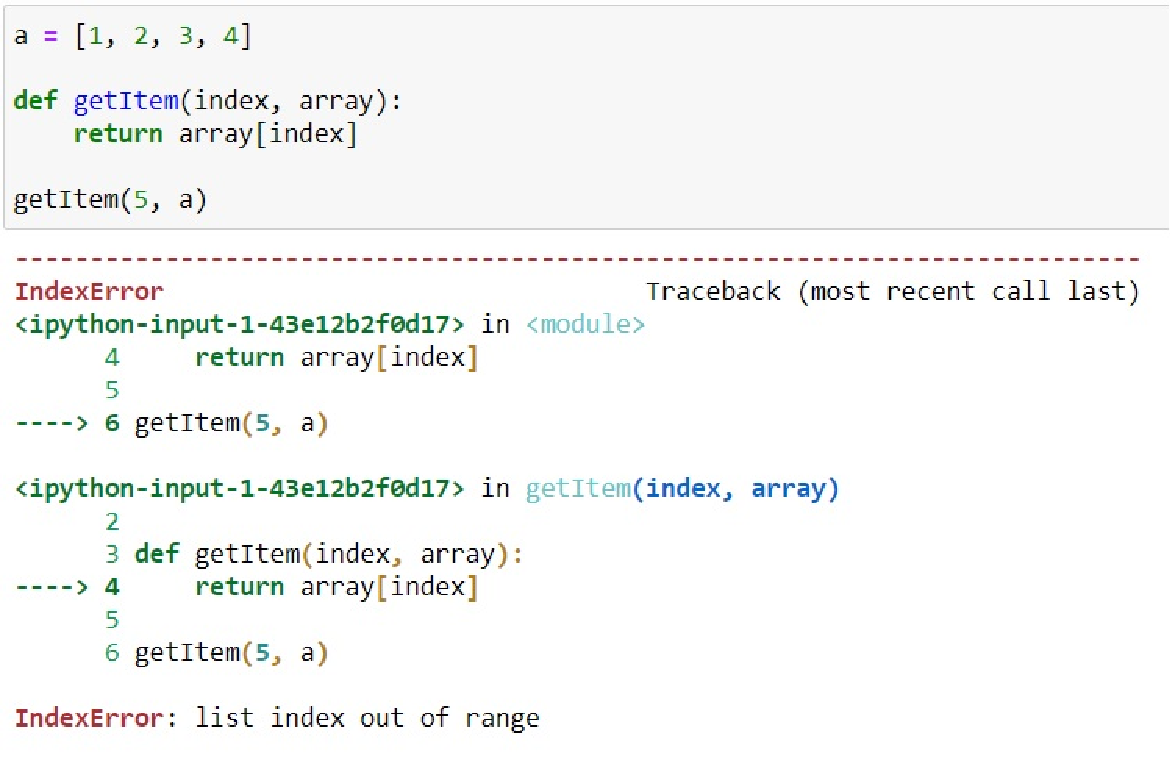
\includegraphics[height=4.5cm, width=6.7cm]{traceback.pdf}
\end{center}


\end{frame}


\begin{frame}
\frametitle{Specifics of Python bugs}

\begin{itemize}
\item if a Python program fails to work, the interpreter usually throws an exception, accompanied with printing out
an error exception report, containing the information about a stack of functions/methods calls,
which cause the program stop;
\item this report can be used for bug localization.
\end{itemize}

\end{frame}


\begin{frame}
\frametitle{Deep learning for bug prediction in Python source code}

\begin{itemize}
\item applying deep learning methodologies (say, Transformers) for natural language processing tasks leads to dramatic improvements;
\item using those methodologies (e.g. graph networks) for finding bugs in Python source code also gives promising results (Allamanis et. al, 2021).
\end{itemize}

\begin{block}{Specifics of deep learning models}
\begin{enumerate}
\item have lots of parameters;
\item require large datasets for their training.
\end{enumerate}
\end{block}

\end{frame}


\section{Related work}


\begin{frame}
\frametitle{Code analysis tasks, underlying known datasets}

Not every known dataset is suitable for training and evaluating deep learning models. Some of the datasets are intended for 
purposes other than fitting neural networks.

\begin{block}{Possible purposes}
\begin{enumerate}
\item automatic test generation: tests must fail on buggy code pieces and work well on fixed pieces;
\item program repair: learn typical patterns of fixing source code and use them to fix unseen code;
\item bug prediction: report if a code piece contains bugs.
\end{enumerate}
\end{block}

\end{frame}

\begin{frame}
\frametitle{Content of the known datasets}

Tasks, underlying datasets, restrict them to contain a specific type of information.
For example, datasets aimed to either automatic test generation or program repair usually contain the so called bugfixes. 

\begin{center}
\vspace{-0.2cm}
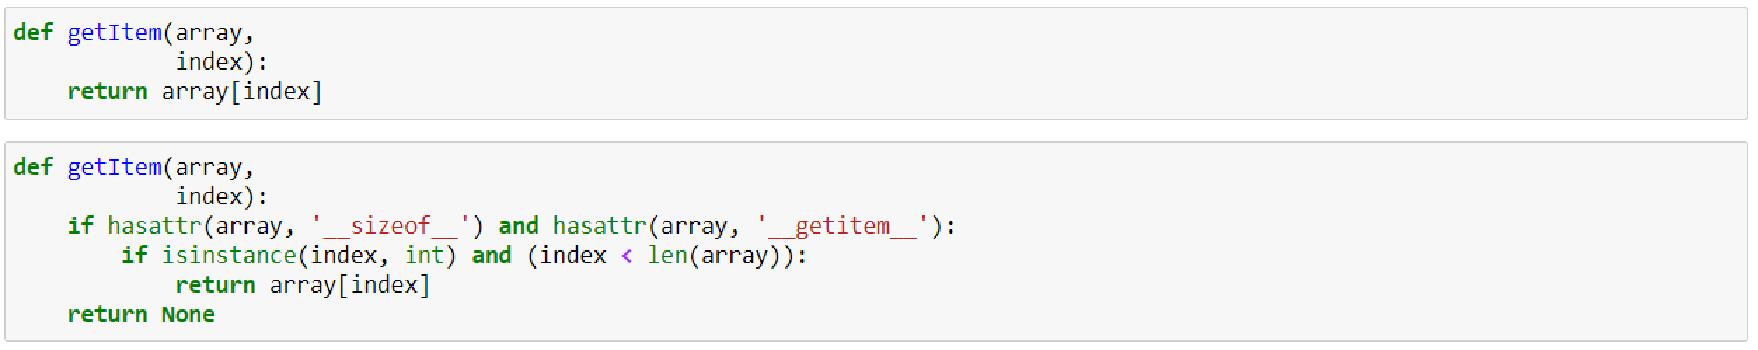
\includegraphics[height=2.2cm, width=10.7cm]{bugfix.pdf}
\end{center}

Each bugfix contains two consequtive versions of the same source code,
where the first piece contains bugs whereas the second one is an immediate fix of those bugs.

\end{frame}


\begin{frame}
\frametitle{Summary of the known datasets}

{\tiny
\begin{table}
\caption{Summary of the known datasets}
\begin{tabular}{|c|c|c|c|c|c|}
\hline
    Name & Language & Granularity & Size & Purpose & Content type \\
\hline
    ManyBugs & C & module & 185 & test generation & bugfix pairs\\
    Defects4J & Java & module & 357 & test generation & bugfix pairs\\
    Bugs.jar & Java & module & 1158 & test generation & bugfix pairs\\
    BugsInPy & Python & file & 493 & test generation & bugfix pairs\\
    GHPR & Java & file & 3026 & bug prediction & bugfix pairs\\
    BugHunter & Java & file/class/snippet & 159k & bug prediction & bugfix pairs \\
    CodRep & Java & snippet & 800k 1 line bugs & program repair & bugfix pairs \\
    ManySStuBs4J & Java & snippet & 153652 1 line bugs & program repair & bugfix pairs \\
    artif. coll. data\footnote{M.Allamanis et al, Self-supervised bug detection and repair, 2021} & Python & snippet & 1M simple bugs& program repair & bugfix pairs \\
\hline
\end{tabular}
\end{table}}

\end{frame}

\section{PyTraceBugs dataset}
\subsection{Features of the PyTraceBugs dataset}
\begin{frame}
\frametitle{Summary of the PyTraceBugs dataset}

{\tiny
\begin{table}
\caption{Summary of the known datasets and our contribution}
\begin{tabular}{|c|c|c|c|c|c|}
\hline
    Name & Language & Granularity & Size & Purpose & Content type \\
\hline
    ManyBugs & C & module & 185 & test gen. & bugfix pairs\\
    Defects4J & Java & module & 357 & test gen. & bugfix pairs\\
    Bugs.jar & Java & module & 1158 & test gen. & bugfix pairs\\
    BugsInPy & Python & file & 493 & test gen. & bugfix pairs\\
    GHPR & Java & file & 3026 & bug pred. & bugfix pairs\\
    BugHunter & Java & file/class/snippet & 159k & bug pred. & bugfix pairs \\
    CodRep & Java & snippet & 800k 1 line bugs & prog. repair & bugfix pairs \\
    ManySStuBs4J & Java & snippet & 153652 1 line examples & prog. repair & bugfix pairs \\
     artif. coll. data\footnote{M.Allamanis et al, Self-supervised bug detection and repair, 2021} & Python & snippet & 1M simple bugs& prog. repair & bugfix pairs \\
    \textbf{PyTraceBugs} & \textbf{Python} & \textbf{snippet} &  \textbf{24k buggy, 5.6M stable} & \textbf{bug pred.} & \textbf{buggy, stable code} \\
\hline
\end{tabular}
\end{table}}

{\small
\begin{itemize}
\item in distinction to the known datasets, PyTraceBugs dataset is collected for the bug prediction task, considered in the form of the binary classification problem with two classes of snippets;
\item 1st class contains buggy code, 2nd class - error-free (or stable) code.
\end{itemize}}
\end{frame}

\begin{frame}
\frametitle{Purpose of the PyTraceBugs dataset}

\begin{block}{Aim of the dataset}
\begin{itemize}
\item PyTraceBugs is a large dataset of Python source code, containing snippets labeled either buggy or correct;
\item the dataset is aimed to pre-training
and fine-tuning complex deep learning models for the bug prediction task.
\end{itemize}
\end{block}

\end{frame}

\begin{frame}
\frametitle{Bugs in the PyTraceBugs dataset}

\begin{block}{Specifics of bugs from the dataset}
Bugs from the dataset manifest themselves in the form of program breaks, accompanied with
error exception reports, containing tracebacks of functions/methods calls, causing their corresponding Python programs stop.
\end{block}

{\tiny
\begin{table}[htbp]
\caption{Most common error types in the dataset}
\begin{center}
\renewcommand{\arraystretch}{1.2}
\begin{tabular}{|c|c|}
\hline
  Error type  & Percentage of snippets (\%) \\
\hline
  AttributeError & 16.6 \\
\hline
  TypeError & 15.9 \\
\hline
  ValueError & 10. \\
\hline
  KeyError & 8.2 \\
\hline
  RuntimeError & 5.5 \\
\hline
  IndexError &  5.3 \\
\hline
  Others &  38.3 \\
\hline
\end{tabular}
\label{tab1}
\end{center}
\end{table}}

\end{frame}

\begin{frame}
\frametitle{Description of the PyTraceBugs dataset}

{\small
\begin{block}{Structure and content of the dataset}
It is split into training, validation and test samples.
\begin{itemize}
\item training and validation samples contain automatically labeled source code from Github repositories;
\item buggy code from those samples is taken from bugfix pairs of snippets, extracted from bugfix commits;
\item error-free code is obtained from stable code of repositories;
\item test sample of 330 snippets contains manually curated buggy code and selected stable code;
\item training and test samples are taken from distinct repositores.
\end{itemize}
\end{block}

In distinction to the dataset of (Allamanis et al, 2021), both training and validation samples 
contain real bugs, i.e. not artificially generated ones.}
\end{frame}

\section{The dataset quality}

\begin{frame}
\frametitle{Confidence of labeling in training and validation samples}

The following ideas are employed to provide high confidence of labeling of snippets into either buggy or correct.

\begin{block}{Approaches to enforce correctness of labeling}
\begin{itemize}
\item source code is extracted from well-respected Github repositories, maintained by experienced developers;
\item buggy snippets are extracted from repositories (bugfix) commits and pull requests, related to Github issues, having bug labels and containing error exception reports on their web pages;
\item snippets of correct code are extracted from highly stable code of repositories;
\end{itemize}
\end{block}
\end{frame}

\begin{frame}
\frametitle{Confidence of labeling in training and validation samples}

To measure amount of noise in the dataset, a percentage is
estimated of buggy snippets, for which changes, introduced in their corresponding fixed versions
from bugfix commits and pull requests, are confined to refactoring.

\begin{block}{Ways to evaluate amount of noise}
\begin{itemize}
\item to obtain a lower bound on the percentage of the
refactoring changes, the rate is estimated of the changess bound to docstrings and
comments (2.6\%);
\item the rate of refactoring changes is estimated manually on a random sample of several hundreds of snippets (10–15\%).
\end{itemize}
\end{block}

\end{frame}

\begin{frame}
\frametitle{Confidence of labeling in the test sample}

Confidence of labeling of snippets in the test sample is made almost 100\%, applying manual validation
by two Python experts.

\begin{block}{Principles, guiding the manual validation}
\begin{itemize}
\item a bug reported on the web page of the corresponding
issue is simple to understand;
\item the reported bug is not dependency, compatibility, or the
regression bug;
\item a fix of the bug introduced into a buggy snippet is also simple;
\item correct snippets are chosen from stable snippets the restriction that
the snippet should be called many times from other snippets.
\end{itemize}
\end{block}


\end{frame}

\begin{frame}
\frametitle{Training predictive models on the dataset}

An alternative way to demonstrate quality of the dataset consists in
building predictive models using its data.

\begin{block}{Details of training predictive model}
\begin{itemize}
\item multi-language pretrained
CodeBERT model is applied to compute embeddings of source code from the dataset;
\item LightGBM classifier is trained on the computed embeddings.
\end{itemize}
\end{block}

{\small
\begin{table}[htbp]
\caption{Results of the prediction experiments on the test sample}
\begin{center}
\renewcommand{\arraystretch}{1.2}
\begin{tabular}{| c | c | c | c |}
\hline
    & Precision & Recall &$F_1$-measure \\
\hline
  correct & 0.61 & 0.99 & 0.76 \\
\hline
  buggy & 0.96 & 0.34 & 0.5 \\
\hline
\end{tabular}
\label{tab8}
\end{center}
\end{table}}

\end{frame}

\section{Conclusion}

\begin{frame}
\frametitle{Conclusion}

{\small
\begin{block}{Basic takeaways}
\begin{itemize}
\item a large labeled dataset is proposed for both training and evaluating of deep learning models
for software bug prediction; 
\item it contains a number of examples of real bugs in the Python source code at the granularity of
snippets, \textit{i.e.}, implementations of functions or methods;
\item confidence in labeling of the snippets in both training and validation samples is about 85\% according to our estimates, whereas it is almost 100\% for the test sample;
\item a model is built on the dataset:
it predicts bugs with precision of 0.96 and recall of 0.34 on the manually validated test sample;
\item the dataset is available at \url{https://github.com/acheshkov/pytracebugs}.
\end{itemize}
\end{block}}

\end{frame}

\begin{frame}

{\Large
\begin{center}
THANK YOU FOR YOUR ATTENTION!
\end{center}}



\end{frame}

\end{document}




